\chapter{Metodología}
\label{chap:metodologia}

\section{Diagnóstico de la Situación Actual}
\textit{[Analizar el estado inicial del sistema, proceso o infraestructura antes de la implementación del proyecto. Describir cómo funciona actualmente y las principales limitaciones técnicas.]}

\section{Área de Estudio}

\begin{table}[htbp]
  \centering
  \caption{Área de estudio.}
  \label{tab:area_estudio}
  \renewcommand{\arraystretch}{1.35}
  \begin{tabular}{|p{0.39\textwidth}|p{0.53\textwidth}|}
    \hline
    \textbf{Dominio:} & \textit{[Indique el dominio académico o científico del proyecto.]} \\
    \hline
    \textbf{Línea de investigación:} & \UTILineaInvestigacion \\
    \hline
    \textbf{Sublínea de investigación:} & \UTISublineaInvestigacion \\
    \hline
    \textbf{Campo:} & Tecnologías de la información y la comunicación (TIC) \\
    \hline
    \textbf{Área:} & \textit{[Defina el área técnica específica del proyecto.]} \\
    \hline
    \textbf{Aspectos:} & \textit{[Describa los procesos, tecnologías o problemas que serán analizados.]} \\
    \hline
    \textbf{Objeto de estudio:} & \textit{[Indique la organización, sistema, proceso o infraestructura objeto del estudio.]} \\
    \hline
    \textbf{Periodo de estudio:} & \textit{[Indique las fechas o el intervalo de tiempo que comprende el estudio.]} \\
    \hline
  \end{tabular}
\end{table}

\section{Metodología de Desarrollo o Implementación}
\textit{[Describir y justificar la metodología empleada según la naturaleza del proyecto, indicando las fases y actividades a ejecutar. Por ejemplo, metodologías ágiles o tradicionales para software, o modelos de diseño, implementación o despliegue para hardware o infraestructura.]}

\section{Técnicas e Instrumentos de Recolección de Información}
\textit{[Describir las técnicas utilizadas para obtener información durante el diagnóstico y la validación del proyecto, tales como entrevistas, encuestas u observación directa.]}

\section{Requerimientos del Proyecto}
\subsection{Requerimientos Funcionales}
\textit{[Enumerar y describir los requerimientos funcionales que la solución debe cumplir.]}
\subsection{Requerimientos No Funcionales}
\textit{[Describir requerimientos relacionados con seguridad, rendimiento, disponibilidad, escalabilidad u otros aplicables.]}

\section{Diseño de la Solución}
\label{sec:diseno_solucion}
\textit{[Describir el diseño técnico de la solución propuesta. Puede incluir arquitectura del sistema o infraestructura, diagramas lógicos y físicos, modelos de datos, componentes o configuraciones técnicas.]}

\section{Justificación Técnica}
\textit{[Argumentar técnicamente la selección de tecnologías, herramientas, plataformas, equipos o servicios utilizados en el proyecto.]}

Ejemplo de cita metodológica: la justificación de decisiones técnicas puede apoyarse en literatura de diseño e implementación de sistemas como \cite{hevner2004design,humble2011devops}.

\subsection{Ejemplo de Imagen 1}
Ejemplo de referencia en el cuerpo del texto: la Imagen~\ref{img:ejemplo_1} puede usarse para documentar evidencia técnica del entorno, componentes o interfaz.

\begin{imagen}[htbp]
  \centering
  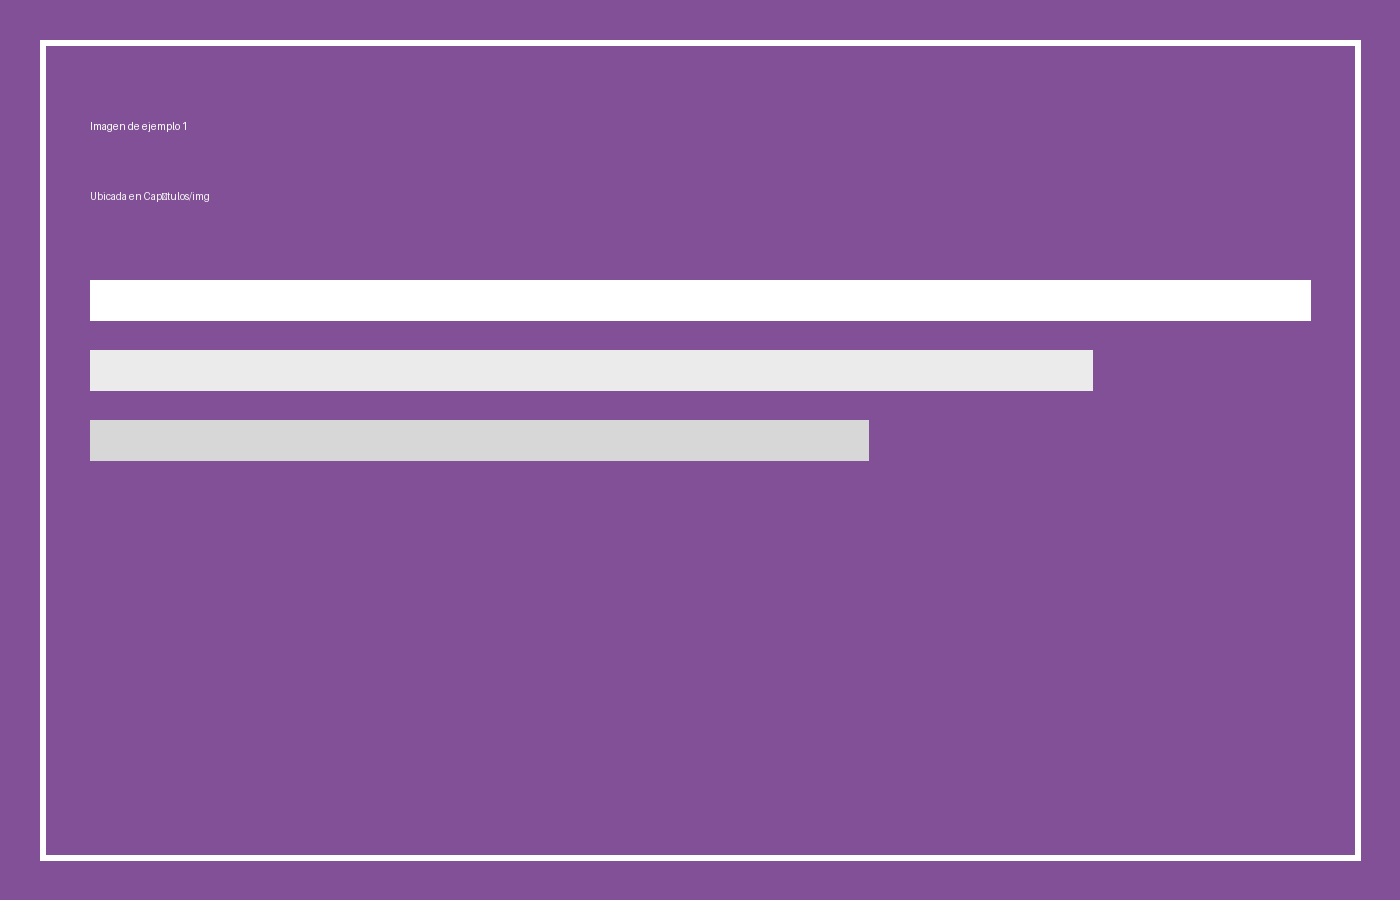
\includegraphics[width=0.80\textwidth]{Capítulos/img/img_ejemplo_1.png}
  \caption{Ejemplo de imagen para documentación visual de infraestructura o evidencias.}
  \label{img:ejemplo_1}
\end{imagen}
\elaboradopor{Estudiante}
\fuente{Captura referencial del proyecto}

\subsection{Ejemplo de Ecuación 1}
Otro ejemplo de referencia: la Ecuación~\ref{eq:disponibilidad} muestra un cálculo típico para validación de disponibilidad del servicio.

\begin{equation}
\label{eq:disponibilidad}
Disponibilidad\,(\%) = \frac{T_{operativo}}{T_{total}} \times 100
\end{equation}
\addeqtolist{Cálculo de disponibilidad del servicio}
